% T0 of the Transport Papers series: the companion primer.
% Correction (2026-09-10, mechanical pass, per Leon): rule 23 misidentified T5 as the printed-version exception. T1 is the exception at Version 3.0; every other paper, T5 included, reads Version 1.0. \date corrected accordingly (was 1.1).
% v1.2 (2026-09-11, interactive session with Leon, Fable 5.1). Section 2's
% on-ramp no longer introduces complex numbers before the geometric product.
% Leon's point: motivating the construction from the complex plane, then
% asking the reader to generalise it, confuses more than it helps; state the
% demand (multiply and divide vectors) and go straight at it. The paragraph
% "The plane already has a better product" and its display of alpha-bar beta
% are removed. In their place, the opening paragraph now states the demand
% (an associative product that keeps the geometry of the pair and can be
% undone), and a new paragraph "What each product throws away, the other
% keeps" observes that the inner and cross products vanish in complementary
% places and between them hold everything about the pair, so a product
% carrying both would have a chance of being invertible. The same two
% questions follow (a dimension-free plane element; the meaning of the sum),
% so the two paragraph headings that answer them are unchanged. Clifford's
% step keeps the complex-number comparison as a one-clause analogy only.
% Example 2.1's closing sentence now presents complex multiplication as a
% consequence of the construction rather than as its motivation. Prose only.
% No mathematics, labels, numbering or claims changed, no new environments.
% verify_T00.py not re-run: script and mathematics untouched.
%   Zenodo pre-flight (2026-09-11, cloud workspace): verify_T00.py 16/16 PASS,
%   re-run against this version, script unchanged; PDF 16 pages.
% v1.1 (2026-09-10, derivation session, Fable 5.1 subagent, per rule 20,
%   series-review repair pass against series_review_2026-09-09.md).
%   Rule 18: Sec 12 (sec:position) now opens "This paper is T0 of the
%   series." and names T1 as "T1 \cite{ButlerT1}" (bibitem already present,
%   title checked against the series list).
%   Rule 17: Example 6.1 (ex:rotor) parenthesis "the machine check below is
%   what caught, and fixed, the wrong sign" -> "the sign is easy to get
%   wrong, and the machine check below verifies it".
%   \date bumped to Version 1.1. Abstract untouched (246 words), no em dashes.
%   Script: verify_T00.py 16/16 PASS, re-run, script unchanged.
%   Compile: pdflatex x2, 16 pages, 0 errors, 0 undefined refs, 0 multiply
%   defined, 0 overfull, no float overflow.
% v1.9 (2026-09-09, interactive session with Leon, Opus 5). One sentence added
% in Section 2, where the geometric product is polarised. The text asserted
% that the antisymmetric part of the product "is the outer product of Figure
% 1", which is an identification of an algebraic object with a geometric one
% already defined, and it asserted it in six words with nothing pointing at
% the check. Two things are now said instead: that the one rule constrains
% only the symmetric half, so the antisymmetric half is new content rather
% than something the axiom determines; and that Example 2.1 is what verifies
% the identification, the antisymmetric part coming out there as the signed
% area times the unit bivector. Leon's point: the reader should be shown what
% licenses the name, not just given it. Prose only. No mathematics, labels,
% numbering or claims changed, and no new environments. Compile: 16 pages,
% 0 errors, 0 undefined, 0 multiply defined, 0 overfull, 0 underfull.
% verify_T00.py 16/16 PASS, unchanged: prose only, the script and the
% mathematics both untouched since v1.7, where it was last run.
% v1.8 (2026-09-09, interactive session with Leon, Opus 5). Section 2's outer
% product no longer stops at the bivector. A new paragraph carries the
% construction up the grades: the outer product is associative, three vectors
% give the trivector as an oriented parallelepiped, k independent vectors give
% the oriented k-dimensional subspace they span weighted by its k-dimensional
% content, and the same antisymmetry that gave a wedge a = 0 makes any
% dependent set vanish, so in n dimensions the sequence ends at k = n with a
% single top object. Section 3's grade paragraph then defines grade by
% reference to those objects rather than introducing them, and names the
% pseudoscalar as the top element Section 2's dependence argument located.
% Leon's point: the reader met the bivector and then met grades built from
% objects never shown. Prose only. No mathematics, labels, numbering or claims
% changed, and no new environments, so every number is untouched. Compile:
% 16 pages, 0 errors, 0 undefined, 0 multiply defined, 0 overfull, 0 underfull.
% verify_T00.py not re-run: unchanged script, unchanged mathematics, 16 PASS
% as recorded at v1.7.
% v1.7 (2026-09-09, interactive session with Leon, Opus 5). Gentler on-ramp
% to Section 2, taking its shape (not its words) from how Doran and Lasenby
% build up to Clifford's product in their Chapter 1: what a product of
% vectors should do, why the inner and cross products fail to do it, the
% plane's invertible product and what it contains, Grassmann's outer
% product, Clifford's sum of the two, and only then the one rule as the
% compact axiom. Section 2 retitled "Products of vectors, and the one rule"
% (label sec:product unchanged). New Figure 1, the oriented parallelogram
% and its reversal (rule 13: this is T0's second figure, the limit); the
% null-cone figure becomes Figure 2, both referenced by label. One sentence
% added to Example 2.1 closing the loop back to the motivating complex
% product. Section 1's plan sentence for Section 2 rewritten, and a skip
% note added for readers who already know the inner and outer products.
% Abstract reworded for the new opening and retrimmed, 246 words.
% NO mathematics, no claims, no labels, no section or lemma numbering
% changed: sections 2 to 13 and toolkit Lemmas 9.1 to 9.6 keep their
% numbers, so T1's and T4's locators into this primer (Section 9, Lemmas
% 9.1 to 9.6, Sections 2 to 4, 5, 6) remain correct. Aux diff: titles,
% page numbers and the new figure only. Compile: 16 pages (was 14), 0
% errors, 0 undefined, 0 multiply defined, 0 overfull, 0 underfull.
% verify_T00.py 16 PASS before and after (run in Claude's workspace).
% v1.6 (2026-09-09, derivation session, Fable 5.1 subagent, per rule 20,
% review-repair pass against T00_review_v1.md, same session). No B findings.
% S1: "combinatorial basis" (Sec 3 closing paragraph) collided with the
% defined term "basis" in the same sentence; now "combinatorial foundation".
% N1: \date bumped from the stale "Version 1.0, August 2026" to 1.6. N2:
% position-in-series sentence, "and, through it, for every later paper" ->
% "in every later paper". N3: "the obstruction in T1's no-go theorem" ->
% "the source of the obstruction in", since T1 uses "obstruction" for the
% cohomology class. No mathematics, labels or numbering changed. Check
% count unchanged: verify_T00.py 16 PASS before and after (no hollow
% check found). Compile: 14 pages, 0 errors, 0 undefined, 0 multiply
% defined, 0 overfull, no float overflow. Numbering frozen: aux diff
% empty. No knock-on for any sibling.
% v1.5 (2026-09-08, prose pass, Fable 5.1 subagent, per project rule 22:
% mannered prose replaced by literal statement, Leon's ruling to replace the
% recurring vocabulary too). Body only; no mathematics, labels, numbering or
% claims changed. Compile: 14 pages, 0 errors, 0 undefined, 0 multiply
% defined; numbering unchanged (aux diff empty); verify_T00.py 16 PASS
% before and after. Abstract trimmed 273 -> 250 words. About 45 sentences.
% Glossary: "owns" -> "assigned to" (4); "at the door" -> "stops where that
% question begins" / "stops here" (2); "costs a sign / a grade involution /
% at the cost of signs" -> "produces" etc. (5); "and nothing more" dropped.
% Non-glossary: "protagonist" -> "central object"; "villains of" -> "the
% obstruction in"; "atom of the whole subject" -> "smallest unit from which
% the whole subject is built"; "the seed is" -> "the basic case is";
% "algebraic shadow" -> "algebraic counterpart"; "workhorse identity" ->
% "identity used most often"; "in disguise" -> "under another name";
% "layers" -> "graded pieces"; "skeleton" -> "basis"; "fate" -> "what
% happens to" (2); "fall apart" -> "decompose"; "type-C story" -> "case";
% "trick" -> "construction" (3); "mandate" -> "uniqueness claim" (2);
% "upstairs/downstairs" -> "in the enlarged space/algebra" / "of V" (5);
% "the door through which the reader should walk into T1" -> "the point at
% which the reader should turn to T1"; "payoff" -> "what this primer takes
% from the model"; "root of everything" -> "paper on which every later
% paper depends"; "downstream" -> "later"; "the hunt done once" ->
% "collects the symbols in one place"; "silently / wordlessly" -> "usually
% without citation / without comment"; "sitting inside" -> "contained in".
% v1.4 (2026-08-25): per Leon, a "Notation at a glance" section added
% (new Section 10, before the reading route): a table of the commonly used
% symbols (perp, oplus, cong, the involutions, the actions, and so on)
% with one-line meanings and pointers to where each is introduced.
% v1.3 (2026-08-24): fresh-eyes review pass. Fixed: the figure's dashed
% level sets (now the true hyperbolas Q = +-1; arrows now v, w themselves);
% honest statement that the classification theorem is cited, not reproved,
% in abstract, Section 1, and toolkit preamble; hyperbolic-pair derivation
% rewritten readably; notation v(v/Q(v)) for the inverse check; cross-term
% remark; unnormalised-rotor and null-rotation precision; Spin^0 dimension
% caveat; metric-faithfulness line in the conformal section; duplicate
% phrases varied; ButlerT1 cited and its bib title punctuation fixed.
% v1.2 (2026-08-24): boundary rebalance per Leon's review. The primer now
% owns only the LANGUAGE of geometric algebra; everything about division
% failing is T1's. Removed: the old Section 6 (three ways division fails)
% and the toolkit's three zero-divisor lemmas (no-inverse, hyperbolic
% pairs, regularity), all returned to T1 with their proofs. Added: Spin^0
% to the rotors section. Toolkit is now six structural lemmas, 9.1 to 9.6.
% v1.1 (2026-08-24): T1's former Section 2 (the classical toolkit) moved here
% per Leon's instruction, as a new toolkit section with complete proofs;
% T1 now restates the lemmas and cites this primer for the proofs.
% v1.0 (2026-08-24): fresh primer written per Leon's instruction, replacing
% the earlier draft. Expository only; not a research contribution; no tier.
% House rules: no em dashes; short abstract; standard series disclaimer;
% T-number identifiers (rule 14); position-in-series section (rule 15);
% prose as simple as possible, but no simpler (rule 16); verification
% imports GA.py (rule 12); diagrams per rule 13 (one figure).
\documentclass[11pt]{article}
\usepackage[margin=1.1in]{geometry}
\usepackage{amsmath,amssymb,amsthm,mathtools,booktabs,array}
\usepackage[dvipsnames]{xcolor}
\usepackage{tikz}
\usepackage[colorlinks=true,linkcolor=MidnightBlue,citecolor=MidnightBlue,urlcolor=MidnightBlue]{hyperref}

\theoremstyle{plain}
\newtheorem{theorem}{Theorem}[section]
\newtheorem{lemma}[theorem]{Lemma}
\theoremstyle{definition}
\newtheorem{example}{Example}[section]

\newcommand{\Cl}{\mathrm{Cl}}
\newcommand{\R}{\mathbb{R}}
\newcommand{\C}{\mathbb{C}}
\newcommand{\HH}{\mathbb{H}}
\newcommand{\Mat}{\mathrm{M}}
\newcommand{\Pin}{\mathrm{Pin}}
\newcommand{\Spin}{\mathrm{Spin}}
\newcommand{\Ad}{\mathrm{Ad}}

\title{\bfseries An Introduction to Geometric Algebra\\[4pt]
  \large\itshape A Primer for the Transport Papers}
\author{Leon Butler\\ \normalsize\href{mailto:lbutler.math@gmail.com}{\texttt{lbutler.math@gmail.com}}\\ \normalsize ORCID: \href{https://orcid.org/0009-0006-4449-5617}{0009-0006-4449-5617}}
\date{Version 1.0, September 2026 \textperiodcentered{} Transport Papers, T0}

\begin{document}
\maketitle

\begin{abstract}
\normalsize
This primer teaches the language of geometric algebra a reader needs before opening the Transport Papers. It motivates the geometric product from what the inner and cross products cannot do, compresses the answer into the one rule $v^{2} = Q(v)$, introduces blades and grades, explains what a signature is and why mixed signatures contain null vectors, presents the two canonical involutions, constructs rotors and the groups $\Pin$ and $\Spin$, and states the mod-8 classification of the real Clifford algebras. It then describes the conformal model, in which the oldest division by zero, $1/0$, is resolved by a projective completion. It closes with a toolkit that proves the classical structural lemmas the series imports: the commutation rule, the twisted adjoint action, the centre and pseudoscalar computations behind the classification (whose induction is cited, not repeated), and the splitting lemma. Every idea is introduced through a worked example, verified by machine in exact arithmetic. Each section names where the series uses its content, so the primer also serves as a reading route. The primer does not treat the failure of division: zero divisors, pseudo-inverses, and the taxonomy of obstructions are assigned entirely to T1, definitions and proofs alike. This is an expository companion, not a research contribution: nothing in it is new, and it carries no epistemic tier. For the mathematics developed properly, see the textbooks cited throughout; for the series' results, see T1, which restates each toolkit lemma it uses and cites this primer for the proof.
\end{abstract}

\medskip
\noindent\textbf{MSC 2020.} Primary 15A66; Secondary 97H60.\\
\textbf{Keywords.} geometric algebra; Clifford algebra; null vector; rotor; conformal model; primer.

\newpage
\textbf{Authorship and disclosure. }The founding idea of the series is the author's: that division by zero in a Clifford algebra should be read not as a prohibition but as a transport into a higher-dimensional algebra, and that the transported division need not be accompanied by an inverse operation. The direction of investigation and the critical review of the results are likewise the author's. The mathematical development and the drafting of the text were carried out in extended collaboration with Claude Fable 5 (Anthropic), an AI system.

\newpage
\section{What this primer is, and is not}\label{sec:scope}

The Transport Papers are a series about what happens where division fails in a Clifford algebra. The series' research papers hold themselves to a strict standard: complete proofs, declared hypotheses, machine verification. That standard leaves no room for slow explanations, and a reader meeting geometric algebra for the first time deserves slow explanations. This primer supplies them.

The plan is short. Section \ref{sec:product} asks what a product of vectors ought to do, shows that the two products of ordinary vector algebra do not do it, and arrives at the geometric product and the single rule that generates it. Section \ref{sec:blades} shows what the resulting algebra looks like inside. Section \ref{sec:signature} explains signature, and why mixed signatures contain the null vectors that are the series' central subject. Section \ref{sec:involutions} introduces the two canonical involutions. Section \ref{sec:rotors} builds rotors, reflections, and the groups $\Pin$ and $\Spin$. Section \ref{sec:clock} states the mod-8 classification. Section \ref{sec:conformal} describes the conformal model and the oldest resolved division by zero. Section \ref{sec:toolkit} collects, with complete proofs, the classical structural lemmas that T1 \cite{ButlerT1} imports. Section \ref{sec:notation} is a one-page table of the symbols the series uses, for a reader who meets one before its section. Section \ref{sec:route} is a reading route through the series. What happens where division fails, the question the series exists to answer, is deliberately not treated here: it is assigned to T1, and Section \ref{sec:signature} stops where that question begins. A reader who already works with the inner and outer products can begin at Section \ref{sec:blades} and use Section \ref{sec:product} only to fix notation.

Three warnings, so that the primer is used correctly. First, it is bounded: no geometric calculus, no applications, no physics. The textbooks do all of that better \cite{Macdonald2010, DoranLasenby2003, DFM2007, HestenesSobczyk1984}. Second, the part used in the series' proofs is exactly one section: the research papers state every fact they use, and the toolkit of Section \ref{sec:toolkit} is where the classical facts among them are proved (save the classification theorem, which the toolkit states with the classical sources cited for its induction). T1 restates the toolkit's lemmas, with their numbers here, and cites this primer for the proofs; everything before the toolkit is a convenience, so that a reader has an easy place to start. Third, it is not new: everything here is classical, and the classical sources are cited section by section \cite{Porteous1995, Lounesto2001, Lam2005, Chevalley1997, ABS1964}.

\section{Products of vectors, and the one rule}\label{sec:product}

Adding vectors causes no trouble. Two displacements compose into a third, the picture and the algebra agree, and there is nothing to explain. What is wanted next is a product: a way of multiplying two vectors that is associative, that keeps the geometry of the pair, and that can be undone, so that knowing $a$ and the product $ab$ recovers $b$. Multiplication and division of vectors, on the same footing as multiplication and division of numbers. That is the whole demand, and it is worth being precise about how the products a reader already knows fall short of it, because the geometric product is built to repair exactly those faults.

Ordinary vector algebra in three dimensions offers two products. The inner product $a \cdot b = |a|\,|b| \cos\theta$ returns a number. It knows lengths and angles, which is most of Euclidean geometry, but it is symmetric in its two arguments and retains nothing about the plane they span. The cross product $a \times b$ returns a vector perpendicular to both, of length $|a|\,|b| \sin\theta$. It does record that plane, but it records it by pointing away from it, and that device is available in three dimensions only: in a plane there is no perpendicular direction to point along, and in four dimensions there are too many, since the vectors orthogonal to a given pair form a plane rather than a line.

Both products have a second limitation, and for this series it is the decisive one. Neither can be undone. Knowing $a$ and the number $a \cdot b$ does not determine $b$, and knowing $a$ and the vector $a \times b$ does not either. There is no division, and no candidate for one. A subject whose question is what happens where division fails cannot start there.

\paragraph{What each product throws away, the other keeps.} The inner product keeps the cosine and discards the plane; the cross product keeps the plane and the sine. Each fails to be invertible exactly where it returns zero, and they return zero in complementary places: $a \cdot b$ vanishes when $b$ is perpendicular to $a$, $a \times b$ when $b$ is parallel to it, and for $a \neq 0$ both vanish only when $b = 0$. Between them they hold everything about the pair. So a single product that carried both pieces at once, the number and the plane, would have lost nothing, and would have a chance of being invertible. That is the product to build, and two questions stand in the way. What should record the plane of $a$ and $b$ in dimensions above three, where no perpendicular vector is available to stand in for it? And what does it mean to add a plane element to a number?

\paragraph{The outer product answers the first.} Grassmann's answer, published in 1844, was to let the plane element be the object itself rather than a perpendicular substitute for it. The \emph{outer product} $a \wedge b$ is the oriented parallelogram spanned by $a$ and $b$: a plane, an area $|a|\,|b| \sin\theta$, and a sense of circulation around it. Exchanging the factors reverses that sense, so the product is antisymmetric,
\[
a \wedge b \;=\; -\, b \wedge a , \qquad \text{and in particular} \qquad a \wedge a \;=\; 0 .
\]
Only the plane, the area and the sense are recorded, not the particular parallelogram: $a \wedge (b + \lambda a) = a \wedge b$ for every scalar $\lambda$, so sliding one edge along the other changes nothing. Because the definition never mentions a perpendicular direction, it makes sense in every dimension. The object it produces is a \emph{bivector}, and it is not a vector. In three dimensions a bivector carries the same information as $a \times b$, which is why the cross product serves so well there, and why it does not generalise.

The construction does not stop at two vectors. The outer product is associative, so three vectors give $a \wedge b \wedge c$, the oriented parallelepiped they span: a three-dimensional subspace, the volume of that parallelepiped, and a handedness. That object is a \emph{trivector}. Four vectors give an oriented four-dimensional volume, and so on, the outer product of $k$ independent vectors representing the oriented $k$-dimensional subspace they span, weighted by its $k$-dimensional content. The antisymmetry that gave $a \wedge a = 0$ makes the outer product of any linearly dependent set vanish, so in an $n$-dimensional space the sequence ends at $k = n$: scalars, vectors, bivectors, trivectors, and upward to a single top object with nothing above it. That ceiling is not a convention. It is the statement that any $n+1$ vectors of an $n$-dimensional space are dependent.

\begin{figure}[ht]
\centering
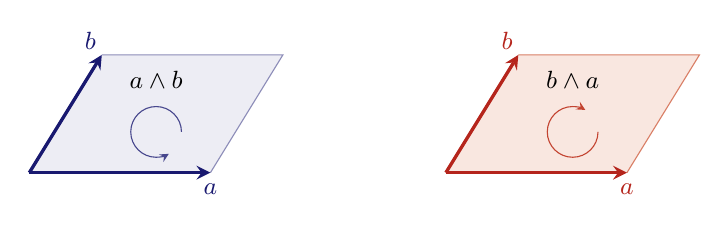
\begin{tikzpicture}[scale=1.15, >=stealth]
  \fill[MidnightBlue!8] (0,0) -- (2,0) -- (2.8,1.3) -- (0.8,1.3) -- cycle;
  \draw[MidnightBlue!50] (2,0) -- (2.8,1.3) -- (0.8,1.3);
  \draw[->, very thick, MidnightBlue] (0,0) -- (2,0) node[below, font=\small] {$a$};
  \draw[->, very thick, MidnightBlue] (0,0) -- (0.8,1.3) node[above left, font=\small, inner sep=1.5pt] {$b$};
  \draw[->, MidnightBlue!80] (1.68,0.45) arc (0:300:0.28);
  \node[font=\small] at (1.4,1.02) {$a \wedge b$};
  \begin{scope}[xshift=4.6cm]
    \fill[BrickRed!8] (0,0) -- (2,0) -- (2.8,1.3) -- (0.8,1.3) -- cycle;
    \draw[BrickRed!50] (2,0) -- (2.8,1.3) -- (0.8,1.3);
    \draw[->, very thick, BrickRed] (0,0) -- (2,0) node[below, font=\small] {$a$};
    \draw[->, very thick, BrickRed] (0,0) -- (0.8,1.3) node[above left, font=\small, inner sep=1.5pt] {$b$};
    \draw[->, BrickRed!80] (1.68,0.45) arc (0:-300:0.28);
    \node[font=\small] at (1.4,1.02) {$b \wedge a$};
  \end{scope}
\end{tikzpicture}
\caption{The outer product. $a \wedge b$ is the oriented parallelogram the two vectors span: a plane, an area $|a|\,|b|\sin\theta$, and a sense of circulation, drawn here as the arrow inside. Taking the factors in the other order reverses the sense, which is what the sign in $b \wedge a = -\,a \wedge b$ records. The shape carries no information: replacing $b$ by $b + \lambda a$ slides the upper edge along the lower one and leaves the product unchanged. Nothing in the definition refers to a direction perpendicular to the plane, so it makes sense in any dimension.}
\label{fig:wedge}
\end{figure}

\paragraph{Clifford's step answers the second.} Keep both parts, and add them:
\[
ab \;=\; a \cdot b \;+\; a \wedge b .
\]
The objection is immediate: a number and a plane element are different kinds of object, and adding them looks like a mistake. The sum claims nothing about numbers and areas being the same kind of thing. It is bookkeeping: the two parts are kept in one symbol because they travel together and the pair is more useful than the pieces, in the way a real part and an imaginary part are kept together in one complex number. Elements that combine objects of several kinds in this way are called \emph{multivectors}.

What the sum buys is division. Take $b = a$: the outer part vanishes, and the product of a vector with itself is the pure number $a \cdot a$, its squared length. So whenever that number is not zero the vector has a two-sided inverse,
\[
a^{-1} \;=\; \frac{a}{a \cdot a} ,
\]
which is what neither the inner nor the outer product could supply alone. Clifford, in 1878, joined Grassmann's outer product to Hamilton's quaternions in exactly this way, and the algebra that results is the subject of this primer.

\paragraph{One rule generates all of it.} That last observation is also the definition. If the square of every vector is a number, then polarising recovers both products, so nothing is lost by taking the one statement as the axiom and deriving the rest.

Start with a real vector space $\mathbb{V}$ carrying a quadratic form $Q$, which assigns to each vector $v$ a number $Q(v)$, its squared length. The \emph{geometric product} is the associative product generated by the vectors of $\mathbb{V}$ subject to one rule:
\[
v^{2} \;=\; Q(v) \qquad \text{for every vector } v .
\]
A vector times itself is a scalar. Everything else follows from this rule and associativity, and the algebra it generates is the \emph{Clifford algebra} $\Cl(\mathbb{V}, Q)$, called the \emph{geometric algebra} of $(\mathbb{V}, Q)$ when one wants to emphasise the geometry.

The two products return at once. Replace $v$ by $a + b$ in the rule and expand:
\[
(a+b)^{2} = a^{2} + ab + ba + b^{2}, \qquad \text{so} \qquad ab + ba \;=\; 2\, a \cdot b ,
\]
where $a \cdot b = \tfrac12\bigl(Q(a+b) - Q(a) - Q(b)\bigr)$ is the inner product obtained by polarising $Q$. So the symmetric part of the geometric product is the inner product, and \emph{orthogonal vectors anticommute}: if $a \cdot b = 0$ then $ab = -ba$. The antisymmetric part is the outer product of Figure \ref{fig:wedge},
\[
a \wedge b \;=\; \tfrac12 (ab - ba), \qquad \text{so that} \qquad ab \;=\; a \cdot b \;+\; a \wedge b ,
\]
which is the decomposition this section arrived at geometrically. The rule constrains only the symmetric half, so the antisymmetric half is new content rather than something the axiom fixes; and that this half is the outer product already defined, and not merely some antisymmetric quantity, is what Example \ref{ex:plane} checks, where it comes out as the signed area of the parallelogram times the unit bivector. The product of two vectors is a scalar plus a bivector, and the bivector represents the oriented plane the two vectors span, weighted by the area of their parallelogram.

\begin{example}[The Euclidean plane]\label{ex:plane}
Let $e_1, e_2$ be an orthonormal basis of the Euclidean plane: $e_1^{2} = e_2^{2} = 1$ and $e_1 \cdot e_2 = 0$, so $e_1 e_2 = -e_2 e_1$. Multiply two general vectors $a = a_1 e_1 + a_2 e_2$ and $b = b_1 e_1 + b_2 e_2$:
\[
ab \;=\; (a_1 b_1 + a_2 b_2) \;+\; (a_1 b_2 - a_2 b_1)\, e_1 e_2 .
\]
The scalar part is the dot product; the coefficient of $e_1 e_2$ is the signed area. One product carries both. Now square the bivector:
\[
(e_1 e_2)^{2} \;=\; e_1 e_2 e_1 e_2 \;=\; - e_1 e_1 e_2 e_2 \;=\; -1 .
\]
The unit bivector of the Euclidean plane squares to $-1$. The even elements $\alpha + \beta\, e_1 e_2$ therefore multiply exactly like complex numbers: the complex plane is contained in the geometric algebra of the real plane, as its even half, and the imaginary unit is the plane's own unit of oriented area. The invertible product the plane has had since the eighteenth century, complex multiplication, is therefore not an ingredient of the construction but a consequence of it.
\end{example}

\paragraph{Where the series uses this.} Everywhere, usually without citation. The commutation rule $ab + ba = 2\,a\cdot b$ is the identity used most often in the proofs of T1, and the observation of Example \ref{ex:plane}, that familiar number systems are geometric algebras under another name, recurs at every scale of the series.

\section{Blades and grades}\label{sec:blades}

Fix an orthogonal basis $e_1, \dots, e_n$ of $\mathbb{V}$. Because orthogonal vectors anticommute and each $e_i^{2}$ is a scalar, any product of basis vectors can be reordered and reduced until each index appears at most once. The surviving products
\[
1, \quad e_i, \quad e_i e_j \ (i<j), \quad e_i e_j e_k \ (i<j<k), \quad \dots, \quad e_1 e_2 \cdots e_n
\]
are the \emph{basis blades}, and they form a linear basis of the algebra: one blade for each subset of the indices, hence
\[
\dim \Cl(\mathbb{V}, Q) \;=\; 2^{n} .
\]
This count holds even when $Q$ is degenerate \cite{Chevalley1997}, a fact the series needs exactly once, in an essential step of one of T1's proofs.

A blade built from $k$ distinct vectors has \emph{grade} $k$, and the grades are exactly the objects Section \ref{sec:product} built: scalars are grade 0, vectors grade 1, the bivectors grade 2, the trivectors grade 3, and so on up to the single top blade $\omega = e_1 e_2 \cdots e_n$, the \emph{pseudoscalar}, which represents the oriented volume of the whole space and is the top element that section's dependence argument located. Grade is basis-independent \cite{Porteous1995}, so the algebra splits into graded pieces, one for each dimension of geometric object it can represent: points of measure, directions, planes, volumes, and so on up to the space itself. The geometric product moves between the grades; the inner and outer products of Section \ref{sec:product} are its grade-lowering and grade-raising parts.

\paragraph{Where the series uses this.} The blade basis and the $2^{n}$ count are the combinatorial foundation of every dimension argument in T1, and the machine verification scripts of the whole series compute in exactly this basis, with exact rational coefficients.

\section{Signature, and the arrival of null vectors}\label{sec:signature}

Over the reals, a nondegenerate quadratic form can be brought to a diagonal shape in which $p$ basis vectors square to $+1$ and $q$ square to $-1$; the pair $(p,q)$ is the \emph{signature}, and it is an invariant (Sylvester's law \cite{Lam2005}). Write $\Cl(p,q)$ for the corresponding algebra. Euclidean space is $(n, 0)$; the spacetime of physics is $(1,3)$: one time direction of positive square, three space directions of negative square.

Signatures with $p, q \geq 1$ are called \emph{mixed}, and something qualitatively new happens there. Positive and negative squares can cancel:
\[
v \;=\; e_1 + e_n, \qquad v^{2} \;=\; e_1^{2} + e_n^{2} \;=\; 1 - 1 \;=\; 0 \qquad (e_1^2 = 1,\ e_n^2 = -1).
\]
(The cross terms $e_1 e_n + e_n e_1 = 2\,e_1 \cdot e_n$ vanish because the basis is orthogonal.) A nonzero vector whose square is zero is called \emph{null} (or isotropic). Null vectors fill a cone, the \emph{null cone}, and in spacetime that cone is the light cone: the null directions are the paths light takes. In a definite signature there are no null vectors at all; $Q(v) = 0$ forces $v = 0$.

A vector with $Q(v) \neq 0$ has the inverse $v^{-1} = v / Q(v)$, since $v\,(v/Q(v)) = v^2/Q(v) = 1$; a null vector has none, and what that failure means, and what can be done about it, is the series' opening question. This primer stops here: the failure of division, its taxonomy, and its repair are assigned to T1, from the first definition onward.

\begin{example}[The hyperbolic plane]\label{ex:hyperbolic}
The smallest mixed signature is $(1,1)$, the \emph{hyperbolic plane}, and it is the smallest unit from which the whole subject is built. Set
\[
v \;=\; \tfrac12 (e_1 + e_2), \qquad w \;=\; \tfrac12 (e_1 - e_2) \qquad (e_1^2 = 1,\ e_2^2 = -1).
\]
Then $v^{2} = w^{2} = 0$: both are null. But their cross terms survive:
\[
vw + wv \;=\; 2\, v\cdot w \;=\; 2\cdot\tfrac14\,(e_1 + e_2)\cdot(e_1 - e_2) \;=\; \tfrac12\bigl(Q(e_1) - Q(e_2)\bigr) \;=\; 1 .
\]
A pair of null vectors with $vw + wv = 1$ is a \emph{hyperbolic pair}, and it satisfies the identity
\[
v\,w\,v \;=\; (1 - wv)\,v \;=\; v - w v^2 \;=\; v .
\]
Multiplying by $v$, then $w$, then $v$ returns $v$ exactly. What this identity means for the failure of division is the opening theme of T1; here it is simply an exact computation worth checking by hand.
\end{example}

\begin{figure}[ht]
\centering
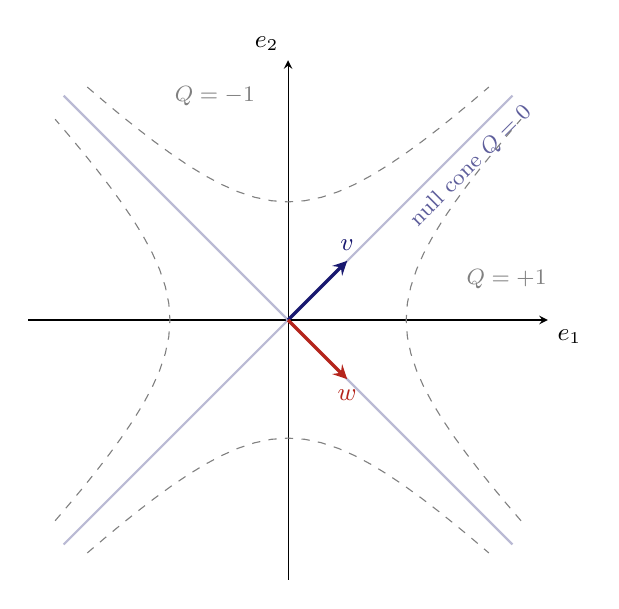
\begin{tikzpicture}[scale=1.5, >=stealth]
  \draw[->, thin] (-2.2,0) -- (2.2,0) node[below right, font=\small] {$e_1$};
  \draw[->, thin] (0,-2.2) -- (0,2.2) node[above left, font=\small] {$e_2$};
  \draw[MidnightBlue!30, thick] (-1.9,-1.9) -- (1.9,1.9);
  \draw[MidnightBlue!30, thick] (-1.9,1.9) -- (1.9,-1.9);
  \node[MidnightBlue!70, font=\footnotesize, rotate=45] at (1.55,1.3) {null cone $Q = 0$};
  \draw[->, very thick, MidnightBlue] (0,0) -- (0.5,0.5) node[above, font=\small] {$v$};
  \draw[->, very thick, BrickRed] (0,0) -- (0.5,-0.5) node[below, font=\small] {$w$};
  \draw[gray, dashed] plot[domain=-1.7:1.7] ({\x}, {sqrt(\x*\x+1)}) plot[domain=-1.7:1.7] ({\x}, {-sqrt(\x*\x+1)});
  \draw[gray, dashed] plot[domain=-1.7:1.7] ({sqrt(\x*\x+1)}, {\x}) plot[domain=-1.7:1.7] ({-sqrt(\x*\x+1)}, {\x});
  \node[gray, font=\footnotesize] at (1.85,0.35) {$Q = +1$};
  \node[gray, font=\footnotesize] at (-0.62,1.9) {$Q = -1$};
\end{tikzpicture}
\caption{The hyperbolic plane $\Cl(1,1)$, drawn in the coordinates of Example \ref{ex:hyperbolic}. The two null lines (light blue) make up the null cone, the set where $Q$ vanishes; the dashed hyperbolas are the level sets $Q = \pm 1$, where every vector is invertible. The hyperbolic pair $v, w$ lies one on each null line, and $vw + wv = 1$. In dimension two the partner on the other line is unique, which is why T1 singles this plane out as the one self-complete mixed signature.}
\label{fig:cone}
\end{figure}

\paragraph{Where the series uses this.} The null cone is the series' central object. T1 classifies what fails there and proves what repairs it; T5 applies the repair to the black-hole singularity, where spacetime's own light cones fold onto a single null direction; and the hyperbolic pair of Example \ref{ex:hyperbolic} reappears in T3 as a fermionic mode, one per rung of an infinite tower.

\section{The two involutions}\label{sec:involutions}

Two canonical symmetries act on every Clifford algebra, both fixed by what they do to vectors.

The \emph{grade involution} $x \mapsto \hat{x}$ sends every vector to its negative, $\hat{v} = -v$, and extends multiplicatively: $\widehat{xy} = \hat{x}\hat{y}$. On a blade of grade $k$ it gives the sign $(-1)^{k}$, so it fixes the even grades and negates the odd ones. It is the algebraic counterpart of the point reflection $x \mapsto -x$.

The \emph{reversion} $x \mapsto \tilde{x}$ fixes every vector, $\tilde{v} = v$, but reverses the order of products: $\widetilde{xy} = \tilde{y}\tilde{x}$. On a blade of grade $k$ it gives the sign $(-1)^{k(k-1)/2}$, the sign produced by reversing $k$ anticommuting factors. It plays the role that transposition plays for matrices and conjugation plays for complex numbers.

One consequence is used constantly. If a vector $v$ is orthogonal to every vector appearing in an element $x$, then moving $v$ past $x$ produces exactly a grade involution:
\[
v\,x \;=\; \hat{x}\,v .
\]
For a single orthogonal vector this is just anticommutation; the general case follows because both sides are multiplicative in $x$.

\paragraph{Where the series uses this.} The commutation rule above is applied dozens of times in T1's proofs, where it is equation (1); the grade involution is the symmetry whose innerness or outerness decides what happens to the split algebras in T1's fusion theorem; and reversion defines the rotor normalisation of Section \ref{sec:rotors}.

\section{Rotors: how the algebra moves things}\label{sec:rotors}

Geometric algebra does not act on vectors through matrices; it acts through its own elements, by a sandwich product. The basic case is the reflection. For an invertible vector $u$, the map
\[
x \;\longmapsto\; -\,u\,x\,u^{-1}
\]
is the reflection of the vector $x$ in the hyperplane orthogonal to $u$: it fixes everything orthogonal to $u$ (which anticommutes past $u$, absorbing the minus sign) and negates $u$ itself. Every isometry of a nondegenerate quadratic space is a product of reflections (the Cartan--Dieudonn\'e theorem \cite{Lam2005}), so products of invertible vectors, called \emph{versors}, reach every element of the orthogonal group $O(p,q)$.

The group formed by versors whose factors are normalised to $Q(u) = \pm 1$ is called $\Pin(p,q)$; its even part, products of an even number of unit vectors, is $\Spin(p,q)$, and covers the rotations. An even versor $R$ with $R\tilde{R} = 1$ is a \emph{rotor}, and it acts by plain conjugation, $x \mapsto R\,x\,R^{-1}$, two reflections making one rotation. One more name the series uses: $\Spin^0(p,q)$ is the \emph{identity component} of $\Spin(p,q)$, the elements joined to $1$ by a continuous path inside the group; in a definite signature of dimension at least two it is all of $\Spin$, while in mixed signature it is a proper subgroup. The precise action of a general versor, including the odd ones, needs a small twist by the grade involution; it is set out and proved in the toolkit (Lemma \ref{tk:tau}).

\begin{example}[A rotation, exactly]\label{ex:rotor}
In the Euclidean plane of Example \ref{ex:plane}, take $R = a - b\,e_1 e_2$ with $a, b$ real, not both zero (a rotor once normalised by $\sqrt{a^2 + b^2}$; the conjugation below ignores the scale). Its reverse is $\tilde{R} = a + b\, e_1 e_2$ and $R\tilde{R} = a^{2} + b^{2}$, so $R^{-1} = \tilde{R}/(a^2 + b^2)$. Conjugating $e_1$:
\[
R\, e_1\, R^{-1} \;=\; \frac{a^{2} - b^{2}}{a^{2} + b^{2}}\, e_1 \;+\; \frac{2ab}{a^{2} + b^{2}}\, e_2 .
\]
The coefficients are the cosine and sine of the double angle of the point $(a,b)$: the rotor rotates $e_1$ towards $e_2$ by $2\arctan(b/a)$, and with $a, b$ rational every entry is exactly rational. (The sign in $R$ is the usual half-angle convention, $R = \cos\tfrac{\theta}{2} - \sin\tfrac{\theta}{2}\, e_1 e_2$; the sign is easy to get wrong, and the machine check below verifies it.) This is the half-angle representation of rotations, and it is why rotors, like quaternions, cover the rotation group twice: $R$ and $-R$ rotate identically.
\end{example}

\begin{example}[A boost, and what it does to a null direction]\label{ex:boost}
In the hyperbolic plane $\Cl(1,1)$, even elements $R = a + b\, e_1 e_2$ have $R\tilde R = a^2 - b^2$, so rotors satisfy $a^{2} - b^{2} = 1$: they are the \emph{boosts}, the hyperbolic rotations of special relativity. Conjugating the null vector $v = \tfrac12(e_1 + e_2)$ of Example \ref{ex:hyperbolic}:
\[
R\,v\,R^{-1} \;=\; (a - b)^{2}\, v \qquad \text{(exactly, using } (a-b)(a+b) = 1\text{)}.
\]
A boost does not move the null direction; it \emph{rescales} it. The null lines are the boost's eigendirections, with reciprocal eigenvalues $(a \mp b)^{2}$. This one computation underlies a great deal of physics: it is why horizons redshift, and in the series it is why the completed algebra at a black-hole singularity carries a preferred one-parameter flow.
\end{example}

\paragraph{Where the series uses this.} The \emph{null rotations}, rotors of the form $1 + vu$ with $v$ null and $u$ orthogonal to $v$, are the source of the obstruction in T1's no-go theorem: they shear every candidate pseudo-inverse of $v$. The boost of Example \ref{ex:boost} becomes, in T5 and T7, the modular flow whose temperature is the Hawking temperature.

\section{The mod-8 classification}\label{sec:clock}

Every real Clifford algebra is a matrix algebra, or a pair of matrix algebras, over $\R$, $\C$ or $\HH$, and which one depends only on $p - q$ modulo 8 \cite{ABS1964, Porteous1995, Lounesto2001}:

\begin{center}
\begin{tabular}{cl@{\qquad}cl}
\toprule
$p-q \bmod 8$ & type & $p-q \bmod 8$ & type \\
\midrule
$0$ & $\Mat_k(\R)$              & $4$ & $\Mat_k(\HH)$ \\
$1$ & $\Mat_k(\R) \oplus \Mat_k(\R)$ & $5$ & $\Mat_k(\HH) \oplus \Mat_k(\HH)$ \\
$2$ & $\Mat_k(\R)$              & $6$ & $\Mat_k(\HH)$ \\
$3$ & $\Mat_k(\C)$              & $7$ & $\Mat_k(\C)$ \\
\bottomrule
\end{tabular}
\end{center}

\noindent In each case the matrix size $k$ is fixed by the dimension count $2^{n}$. The small algebras are worth knowing by name: $\Cl(1,0) \cong \R \oplus \R$ (residue 1, split), $\Cl(0,1) \cong \C$ (residue 7), $\Cl(2,0) \cong \Cl(1,1) \cong \Mat_2(\R)$ (residues 2 and 0), $\Cl(0,2) \cong \HH$ (residue 6), $\Cl(0,3) \cong \HH \oplus \HH$ (residue 5), and the spacetime algebra $\Cl(1,3) \cong \Mat_2(\HH)$ (residue 6). The doubled rows, residues 1 and 5, are the \emph{split} algebras, the ones that decompose into two ideals; what that means for division is T1's type-C case.

The table repeats with period 8, and the repetition has a mechanism: adding one $(+1)$ and one $(-1)$ direction at once leaves $p - q$ unchanged and doubles the matrix size,
\[
\Cl(p{+}1,\, q{+}1) \;\cong\; \Mat_2\bigl(\Cl(p,q)\bigr),
\]
the $(1,1)$-periodicity theorem. This matters here, because the added $(+1,-1)$ pair spans exactly a hyperbolic plane: the unit of Example \ref{ex:hyperbolic} is also the unit of the classification's own periodicity.

\paragraph{Where the series uses this.} T1 imports the pieces of this table its theorems rest on (the proofs are in Section \ref{sec:toolkit}), and turns the classification into a state machine, the mod-8 clock: its Rule 1 fixes the residue, its Rule 2 moves it off the split rows exactly once. The tower of T3 is the $(1,1)$-periodicity iterated, one hyperbolic plane, and one fermionic mode, per step.

\section{The conformal model, and the oldest division by zero}\label{sec:conformal}

The final construction is the one the series turns into a principle. Take a quadratic space $(\mathbb{V}, Q)$ of signature $(p,q)$ and adjoin two extra directions $e_+, e_-$ with $e_+^{2} = +1$, $e_-^{2} = -1$: one hyperbolic plane, giving $\Cl(p{+}1, q{+}1)$. Out of the new plane build the null pair
\[
n_0 = \tfrac12(e_- - e_+), \qquad n_\infty = e_- + e_+ ,
\]
representing the origin and the point at infinity, and represent each point $x \in \mathbb{V}$ by the vector
\[
X(x) \;=\; n_0 + x + \tfrac12 Q(x)\, n_\infty .
\]
A short computation gives $X(x)^{2} = 0$: every point of the space is represented by a \emph{null} vector in the enlarged space, determined up to scale, so points become null rays on a quadric. The lift also remembers the geometry exactly, since $X(x) \cdot X(y) = -\tfrac12\,Q(x - y)$. This is the \emph{conformal model} of geometric algebra \cite{Hestenes2001, DFM2007, DoranLasenby2003}, and its power is that the conformal transformations of $\mathbb{V}$, inversions included, all become sandwich products in the enlarged algebra.

What this primer takes from the model is the oldest division by zero. Take the real line, $\mathbb{V} = \R$ with $Q(x) = x^{2}$. The reciprocal $x \mapsto 1/x$ fails at the origin. In the enlarged space, the quadric is a circle, the projective line $\R P^{1}$ in homogeneous coordinates $[\,x : s\,]$, and the reciprocal becomes the linear swap $[\,x : s\,] \mapsto [\,s : x\,]$, which is total: it never fails anywhere. At the origin it gives $[\,0 : 1\,] \mapsto [\,1 : 0\,]$, the point at infinity. Division by zero has an answer; the answer simply is not a real number, and it lies in the completion. Nothing here is new: this is the nineteenth-century projective resolution of $1/0$, the same construction that makes M\"obius maps $z \mapsto (az+b)/(cz+d)$ total on the Riemann sphere.

What the series adds, and this is the point at which the reader should turn to T1, is a uniqueness claim: for a general quadratic space this completion is not one convenient construction among many but the \emph{unique minimal} resolution of the null cone's division failure, the repair of the element itself being provably impossible. The construction becomes a theorem.

\paragraph{Where the series uses this.} T1 proves the uniqueness claim. T5 applies it to spacetime: the ascent $\Cl(1,3) \to \Cl(2,4)$ forced at the black-hole singularity lands on the conformal algebra of spacetime, whose spinors are Penrose's twistors (T9).

\section{The toolkit: the classical lemmas the series imports}\label{sec:toolkit}

Everything so far was informal on purpose. This closing section is not: it states, and proves in full (the classification theorem alone is stated with the classical sources cited for its induction), the classical structural facts that T1's theorems rest on, the facts about the algebra's symmetries and structure that belong to the language rather than to the failure of division. T1 restates each of them, with its number here, and cites this section for the proof. The zero-divisor lemmas T1 also needs (that a null vector has no inverse, that null vectors come in hyperbolic pairs, that regularity localises zero divisors at idempotents) are stated and proved in T1 itself, because the failure of division is that paper's subject, not this one's. Nothing in this section is new; the sources are the ones cited throughout \cite{Porteous1995, Lounesto2001, Lam2005, Chevalley1997, ABS1964}.

Throughout, $(\mathbb{V}, Q)$ is a finite-dimensional real quadratic space with polarisation $a \cdot b = \tfrac12(Q(a+b) - Q(a) - Q(b))$, nondegenerate unless stated otherwise, of signature $(p,q)$ with $n = p + q$.

\begin{lemma}[The commutation rule]\label{tk:commutation}
If the element $x$ lies in the subalgebra generated by vectors orthogonal to a vector $v$, then
\begin{equation}\label{eq:tkcommutation}
v\,x = \hat{x}\,v, \qquad x\,v = v\,\hat{x} .
\end{equation}
\end{lemma}

\begin{proof}
For a single orthogonal vector $u$ this is the anticommutation $vu = -uv = \hat{u}v$ of Section \ref{sec:product}, and scalars commute with everything while being fixed by $\hat{\cdot}$. The general case follows because both sides of $vx = \hat{x}v$ are multiplicative in $x$ ($v(xy) = \hat{x}vy = \hat{x}\hat{y}v = \widehat{xy}\,v$, using that $\hat{\cdot}$ is an automorphism) and linear in $x$. The second identity is the first read from the other side, since $\hat{\cdot}$ is an involution.
\end{proof}

\begin{lemma}[The twisted adjoint action]\label{tk:tau}
Let $g = u_1 \cdots u_k$ be a versor and define, on the whole algebra,
\begin{equation}\label{eq:tktau}
\tau_g(x) \;=\;
\begin{cases}
\,g\, x\, g^{-1} & g \text{ even},\\[2pt]
\,g\, \hat{x}\, g^{-1} & g \text{ odd}.
\end{cases}
\end{equation}
Then each $\tau_g$ is an algebra automorphism, and on vectors it restricts to the twisted adjoint $\Ad_g(x) = \hat{g} x g^{-1}$. For a single invertible vector $u$,
\[
\Ad_u(x) \;=\; -\,u x u^{-1} \;=\; x - 2\,\frac{x \cdot u}{Q(u)}\,u ,
\]
the reflection in the hyperplane orthogonal to $u$; consequently $g \mapsto \Ad_g$ maps $\Pin(p,q)$ onto $O(p,q)$ with kernel $\{\pm 1\}$.
\end{lemma}

\begin{proof}
For even $g$, $\tau_g$ is plain conjugation, an automorphism. For odd $g$,
\[
\tau_g(x)\,\tau_g(y) \;=\; g\hat{x}g^{-1}g\hat{y}g^{-1} \;=\; g\,\hat{x}\hat{y}\,g^{-1} \;=\; g\,\widehat{xy}\,g^{-1} \;=\; \tau_g(xy),
\]
and $\tau_g(1) = 1$, so $\tau_g$ is again an automorphism; naive conjugation by an odd versor is not vector-preserving, and the twist by $\hat{\cdot}$ is the standard repair. On a vector $x$, for odd $g$ we have $\hat{g} = -g$, so $\tau_g(x) = g\hat{x}g^{-1} = -gxg^{-1} = \hat{g}xg^{-1} = \Ad_g(x)$; for even $g$, $\hat{g} = g$ and the two agree at once. For a single invertible vector $u$, split $x = x_{\parallel} + x_{\perp}$ with $x_{\parallel} = \dfrac{x \cdot u}{Q(u)}\,u$ along $u$ and $x_{\perp}$ orthogonal to $u$: then $u x_{\parallel} u^{-1} = x_{\parallel}$ (parallel vectors commute) and $u x_{\perp} u^{-1} = -x_{\perp}$ (orthogonal vectors anticommute), so $-uxu^{-1} = x_{\perp} - x_{\parallel} = x - 2x_{\parallel}$, the stated reflection. Cartan--Dieudonn\'e \cite{Lam2005, Porteous1995} writes every element of $O(p,q)$ as a product of reflections, giving surjectivity; the kernel computation is classical \cite{Porteous1995}.
\end{proof}

\begin{theorem}[Classification of the real Clifford algebras]\label{tk:classification}
Let $d \equiv p - q \pmod 8$. Then $\Cl(p,q)$ is isomorphic, as a real associative algebra, to the entry of the table of Section \ref{sec:clock}: $\Mat_k(\R)$ for $d \in \{0, 2\}$, $\Mat_k(\C)$ for $d \in \{3, 7\}$, $\Mat_k(\HH)$ for $d \in \{4, 6\}$, $\Mat_k(\R) \oplus \Mat_k(\R)$ for $d = 1$, and $\Mat_k(\HH) \oplus \Mat_k(\HH)$ for $d = 5$, with $k$ fixed in each case by $\dim_\R \Cl(p,q) = 2^n$. In particular $\Cl(p,q)$ is simple except when $p - q \equiv 1 \pmod 4$, where it is the direct sum of two isomorphic simple algebras.
\end{theorem}

\begin{proof}
This is the theorem of the classical sources \cite{ABS1964, Porteous1995, Lounesto2001}, assembled from the low-dimensional isomorphisms of Section \ref{sec:clock} and the $(1,1)$-periodicity $\Cl(p{+}1,q{+}1) \cong \Mat_2(\Cl(p,q))$; we do not repeat their induction here.
\end{proof}

\begin{lemma}[The centre]\label{tk:center}
For $n \geq 1$, the centre of $\Cl(p,q)$ is $\R \cdot 1$ if $n$ is even, and $\R \cdot 1 \oplus \R \cdot \omega$ if $n$ is odd, where $\omega = e_1 e_2 \cdots e_n$ is the pseudoscalar.
\end{lemma}

\begin{proof}
For a basis blade $e_I$ of grade $k$ and a generator $e_j$, anticommuting $e_j$ through $e_I$ gives
\[
e_j e_I = (-1)^{k - [j \in I]}\, e_I e_j,
\]
where $[j \in I]$ is $1$ or $0$: passing $e_j$ across each factor of $e_I$ produces a sign except at the factor $e_j$ itself, if present. Every generator $e_j$ is invertible ($e_j^2 = \pm 1$), and conjugation by $e_j$ maps each basis blade to itself up to the sign above: $e_j\, e_I\, e_j^{-1} = (-1)^{k - [j \in I]}\, e_I$. A central element is fixed by every such conjugation, so each blade coefficient $\lambda_I \neq 0$ must have sign $+1$ against every $j$. Fix a blade $e_I$ with $\lambda_I \neq 0$ and $0 < k < n$, and choose $j \in I$ and $j' \notin I$ (possible since $0 < k < n$): the condition from $e_j$ is $(-1)^{k-1} = 1$ ($k$ odd), from $e_{j'}$ it is $(-1)^{k} = 1$ ($k$ even), and the two are incompatible. Hence $\lambda_I = 0$ for all $0 < k < n$, and any central $x$ lies in $\R \oplus \R\omega$. Finally $\omega$ itself: taking $k = n$, the condition from any $e_j$ (all $j \in I$) is $(-1)^{n-1} = 1$, i.e.\ $n$ odd. For $n$ even the centre is therefore $\R$; for $n$ odd, $\R \oplus \R\omega$.
\end{proof}

\begin{lemma}[The sign of $\omega^2$]\label{tk:omegasq}
$\displaystyle \omega^2 = (-1)^{\tfrac{n(n-1)}{2}} (-1)^q = (-1)^{\tfrac{(p-q)(p-q-1)}{2}}$. In particular $\omega^2 = +1$ if and only if $p - q \equiv 0$ or $1 \pmod 4$.
\end{lemma}

\begin{proof}
Reversion reverses the factors of $\omega$, which takes $\binom{n}{2} = \tfrac{n(n-1)}{2}$ transpositions of orthogonal (hence anticommuting) generators: $\tilde{\omega} = (-1)^{n(n-1)/2}\,\omega$. On the other hand $\omega \tilde{\omega} = e_1 \cdots e_n\, e_n \cdots e_1 = e_1^2 \cdots e_n^2 = (+1)^p(-1)^q$, collapsing from the inside out. Combining, $\omega^2 = (-1)^{n(n-1)/2}(-1)^q$. For the second form set $m = p - q$, so $n \equiv m \pmod 2$ and $q = (n-m)/2$; the exponent is
\[
\frac{n(n-1)}{2} + \frac{n-m}{2} \;=\; \frac{n^2 - m}{2},
\qquad
\frac{n^2 - m}{2} - \frac{m^2 - m}{2} \;=\; \frac{(n-m)(n+m)}{2} \;=\; 2pq,
\]
an even integer, so the exponent is congruent mod 2 to $\tfrac{m^2 - m}{2} = \tfrac{m(m-1)}{2}$. Hence $\omega^2 = (-1)^{m(m-1)/2}$, and $m(m-1)/2$ is even exactly for $m \equiv 0, 1 \pmod 4$.
\end{proof}

\begin{lemma}[Splitting along a hyperbolic plane]\label{tk:split}
Let $\mathbb{V}' = H_0 \perp U'$ be an orthogonal decomposition of a real quadratic space, with $H_0$ a hyperbolic plane spanned by a hyperbolic pair $(v, w_0)$ (a pair of null vectors with $v w_0 + w_0 v = 1$, Example \ref{ex:hyperbolic}); the form on $U'$ may be degenerate. Then:
\begin{enumerate}
\item $\{1, v, w_0, v w_0\}$ is a linear basis of $\Cl(H_0)$, and every element of $\Cl(\mathbb{V}')$ admits a \emph{unique} expansion
\[
\sigma \;=\; \alpha + v\beta + w_0\gamma + v w_0\,\delta, \qquad \alpha, \beta, \gamma, \delta \in \Cl(U').
\]
\item Left multiplication by $v$ is injective on $\Cl(U')$.
\end{enumerate}
\end{lemma}

\begin{proof}
(1) $\Cl(H_0)$ has dimension $4$; the elements $1, v, w_0$ are independent (grades $0$ and $1$), and $v w_0 = v \cdot w_0 + v \wedge w_0 = \tfrac12 + v \wedge w_0$ has a nonzero grade-$2$ component, so the four are a basis. Every vector of $U'$ is orthogonal to $H_0$, hence anticommutes with $v$ and $w_0$; consequently any product of generators of $\Cl(\mathbb{V}')$ can be reordered, changing only signs, into (an element of $\Cl(H_0)$)$\,\times\,$(an element of $\Cl(U')$). The products of the four basis elements of $\Cl(H_0)$ with the $2^{\dim U'}$ basis blades of $\Cl(U')$ therefore span $\Cl(\mathbb{V}')$, and since their number $4 \cdot 2^{\dim U'} = 2^{\dim \mathbb{V}'}$ equals $\dim \Cl(\mathbb{V}')$ (valid whether or not $Q'|_{U'}$ is degenerate, by the count of Section \ref{sec:blades} \cite{Chevalley1997}), they form a basis. This is the graded tensor decomposition $\Cl(A \perp B) \cong \Cl(A)\,\hat{\otimes}\,\Cl(B)$ \cite{Lam2005} in coordinates.

(2) For $x \in \Cl(U')$, the element $vx$ \emph{is} an expansion of the form in (1), with $\beta = x$ and $\alpha = \gamma = \delta = 0$. By uniqueness, $vx = 0$ forces $x = 0$.
\end{proof}

\paragraph{Where the series uses this.} These are the structural facts T1's Section 2 imports; T1's proofs invoke them by the numbers above. The commutation rule is the main tool of T1's no-go theorem; the splitting lemma is the essential step announced in Section \ref{sec:blades}; and the centre and $\omega^2$ computations decide what happens to the split algebras in T1's fusion theorem.

\section{Notation at a glance}\label{sec:notation}

Every symbol below is introduced somewhere in this primer or in T1, but a reader should not have to search for the introduction. This table collects the symbols in one place. The section column names where the symbol is first explained; symbols marked T1 belong to that paper's own constructions and are listed here so that the whole series can be read with one table at hand.

\begin{center}
\small
\begin{tabular}{cl>{\raggedright\arraybackslash}p{7.0cm}c}
\toprule
Symbol & Name & What it means & Where \\
\midrule
$Q(v)$ & quadratic form & the squared length the geometry assigns to $v$; the algebra's one rule is $v^2 = Q(v)$ & \S\ref{sec:product} \\
$a \cdot b$ & inner product & the symmetric part of the product, $\tfrac12(ab + ba)$; $a \cdot b = 0$ says $a$ and $b$ are orthogonal & \S\ref{sec:product} \\
$a \wedge b$ & outer product & the antisymmetric part, $\tfrac12(ab - ba)$; the oriented plane spanned by $a$ and $b$ & \S\ref{sec:product} \\
$\Cl(p,q)$ & Clifford algebra & the algebra of a space with $p$ directions of square $+1$ and $q$ of square $-1$ & \S\ref{sec:signature} \\
$\Cl(\mathbb{V}, Q)$ & the same, by space & the algebra named by the specific space rather than its signature; the form used when $Q$ may be degenerate & \S\ref{sec:product} \\
$\omega$ & pseudoscalar & the top blade $e_1 e_2 \cdots e_n$, the oriented volume of the whole space & \S\ref{sec:blades} \\
$\hat{x}$ & grade involution & the sign $(-1)^k$ on grade $k$: fixes even grades, negates odd ones & \S\ref{sec:involutions} \\
$\tilde{x}$ & reversion & reverses the order of factors in any product of vectors; sign $(-1)^{k(k-1)/2}$ on grade $k$ & \S\ref{sec:involutions} \\
$\perp$ & orthogonal sum & $\mathbb{V} = A \perp B$: the space splits into two parts, every vector of one orthogonal to every vector of the other; $W^{\perp}$ is the set of vectors orthogonal to all of $W$ & \S\ref{sec:toolkit} \\
$\oplus$ & direct sum & an algebra falling into two independent blocks, multiplied componentwise; the two blocks annihilate each other & \S\ref{sec:clock} \\
$\cong$ & isomorphic & the same structure under a renaming of elements & \S\ref{sec:clock} \\
$\Mat_k(\mathbb{F})$ & matrix algebra & the $k \times k$ matrices with entries in $\mathbb{F}$ & \S\ref{sec:clock} \\
$\R,\ \C,\ \HH$ & the three fields & the real numbers, the complex numbers, and the quaternions & \S\ref{sec:clock} \\
$\Pin,\ \Spin,\ \Spin^0$ & the versor groups & normalised versors; their even part; its identity component & \S\ref{sec:rotors} \\
$\Ad_g,\ \tau_g$ & the twisted actions & how a versor $g$ moves vectors ($\Ad$) and general elements ($\tau$) & Lem.\ \ref{tk:tau} \\
$n_0,\ n_\infty$ & origin and infinity & the null pair of the conformal model, representing the origin and the point at infinity & \S\ref{sec:conformal} \\
$X(x)$ & conformal lift & the null vector in the enlarged space that represents the point $x$ of $\mathbb{V}$ & \S\ref{sec:conformal} \\
$p - q \bmod 8$ & clock residue & the number that decides which entry of the classification table an algebra is & \S\ref{sec:clock} \\
$e^2 = e$ & idempotent & a projection; apart from $0$ and $1$, always a zero divisor & T1 \\
$v\sigma v = v$ & pseudo-inverse & the standard weakened substitute for an inverse when none exists & T1 \\
\bottomrule
\end{tabular}
\end{center}

\paragraph{Where the series uses this.} Everywhere, without comment. A reader who bookmarks one page of the primer should bookmark this one.

\section{A reading route}\label{sec:route}

The series is eighteen papers, T0 to T17, in six arcs. This primer is T0. The algebra arc is T1 to T4: T1 proves the transport principle, the taxonomy of division failures and the minimal repair of each, and is the paper on which every later paper depends; T2 is a short applied note (projective geometric algebra completes to conformal); T3 iterates the ascent into a tower and finds second quantisation at the top; T4 does the sheaf theory needed when the failure happens along a locus rather than at a point. The black-hole arc is T5 and T6: T5 runs the whole method on the Schwarzschild singularity and dissolves the information paradox as a category error; T6 is its mathematical-relativity companion. Then come the quantum companions T7 and T8 (Hawking radiation; black-hole entropy and scrambling), the identification arc T9 and T10 (twistors; dark energy and the action of gravity), the matter arc T11 to T15 (the origin of mass; the Standard Model; quark and lepton families; dark matter; neutrino masses), and the synthesis T16 and T17 (quantum mechanics and general relativity from one relation; the capstone survey).

A reader new to all of it should read this primer, then T1, then T5, and then follow their own interests; T17, the capstone, is a map of the whole series with the status of every claim.

\section{Position in the series}\label{sec:position}

This paper is T0 of the series.

\emph{This paper relies on:} nothing in the series. It is expository, and its sources are the cited textbooks.

\emph{Papers that rely on this one:} T1 \cite{ButlerT1}, for the toolkit. T1 \cite{ButlerT1} restates each lemma of Section \ref{sec:toolkit} under its own numbering and cites this primer for the proofs, so the toolkit is used in the proofs of the series' first research paper and, through it, in every later paper. The rest of the primer is a convenience, a place to send a reader meeting geometric algebra for the first time.

\section{Machine verification}\label{sec:verification}

Although this primer proves nothing new, its worked examples are computations, and the series' standard is that computations are machine-checked. The script \texttt{verify\_T00.py}, deposited alongside this paper, imports the series' shared exact-arithmetic library \texttt{GA.py} and verifies, in exact rational arithmetic with no floating point: the geometric-product identities of Example \ref{ex:plane}, including $(e_1e_2)^2 = -1$ and the complex-multiplication table of the even subalgebra; the dimension count $2^{n}$ for $n \leq 6$; the hyperbolic-pair identities of Example \ref{ex:hyperbolic}; the commutation rule $vx = \hat{x}v$ and the involution signs on all blades for $n \leq 5$; the reflection and rotor formulas of Section \ref{sec:rotors}, with the exact rational rotation of Example \ref{ex:rotor} and the boost eigenvalue $(a-b)^{2}$ of Example \ref{ex:boost}; the pseudoscalar squares and centre dimensions behind the table of Section \ref{sec:clock}, exhaustively for $n \leq 6$; the conformal lift's nullity, metric faithfulness, and the total swap on the projective line, including $1/0 = \infty$; and the computational content of the toolkit: the splitting lemma's unique expansion and the injectivity of null multiplication (Lemma \ref{tk:split}), and the twisted adjoint action's multiplicativity and reflection formula (Lemma \ref{tk:tau}). Sixteen checks, all passing.

\begin{thebibliography}{99}

\bibitem{Macdonald2010}
A.~Macdonald,
\emph{Linear and Geometric Algebra},
CreateSpace (2010).

\bibitem{DoranLasenby2003}
C.~Doran and A.~Lasenby,
\emph{Geometric Algebra for Physicists},
Cambridge University Press (2003).

\bibitem{DFM2007}
L.~Dorst, D.~Fontijne and S.~Mann,
\emph{Geometric Algebra for Computer Science},
Morgan Kaufmann (2007).

\bibitem{HestenesSobczyk1984}
D.~Hestenes and G.~Sobczyk,
\emph{Clifford Algebra to Geometric Calculus},
Reidel, Dordrecht (1984).

\bibitem{Hestenes2001}
D.~Hestenes,
Old wine in new bottles: a new algebraic framework for computational geometry,
in \emph{Geometric Algebra with Applications in Science and Engineering},
Birkh\"auser, Boston (2001).

\bibitem{Porteous1995}
I.~R.~Porteous,
\emph{Clifford Algebras and the Classical Groups},
Cambridge University Press (1995).

\bibitem{Lounesto2001}
P.~Lounesto,
\emph{Clifford Algebras and Spinors}, 2nd ed.,
Cambridge University Press (2001).

\bibitem{Lam2005}
T.~Y.~Lam,
\emph{Introduction to Quadratic Forms over Fields},
American Mathematical Society (2005).

\bibitem{Chevalley1997}
C.~Chevalley,
\emph{The Algebraic Theory of Spinors and Clifford Algebras},
Collected Works, Vol.~2, Springer, Berlin (1997).

\bibitem{ABS1964}
M.~F.~Atiyah, R.~Bott and A.~Shapiro,
Clifford modules,
\emph{Topology} \textbf{3} (1964), suppl.~1, 3--38.

\bibitem{ButlerT1}
L.~Butler,
\emph{The Transport Principle: Total Division in Clifford Algebras via Minimal Completion},
Transport Papers T1 (2026).

\end{thebibliography}

\end{document}
